\documentclass[a4paper,11pt]{report} % ligne de classe
% preambule

\usepackage[utf8]{inputenc}
\usepackage[T1]{fontenc}
\usepackage[frenchb]{babel}
\usepackage{textcomp} 
\usepackage[top=3cm,left=3cm,right=3cm,bottom=2cm]{geometry}
\usepackage{lmodern}
\usepackage{sectsty}
%\usepackage{nicefrac}
\usepackage{graphicx}
\usepackage{lastpage}
\usepackage{fancyhdr}
\usepackage{amsmath}
\usepackage{amssymb}
\usepackage{amsfonts}
\usepackage{capt-of}
\usepackage{caption}
\usepackage{tikz}
\usepackage{multirow}
    
    
\usepackage{fancyvrb} % pour forcer les verbatim sur une seule page
\usepackage{url}
    
\usepackage{subfigure}
%\usepackage{subcaption}
    
%\newcommand\matlab{MATLab\textsuperscript{\textregistered}}

\renewcommand{\baselinestretch}{1.1}

\usepackage[colorinlistoftodos]{todonotes}

%\usepackage{cite} 
\usepackage[round,authoryear,numbers]{natbib}


\usepackage{hyperref}
\hypersetup{
     colorlinks   = true,
     citecolor    = blue!90
}



\begin{document} % début du doc
% corps du doc

\begin{titlepage}

\newcommand{\HRule}{\rule{\linewidth}{0.5mm}} % Defines a new command for the horizontal lines, change thickness here

\center % Center everything on the page
 
%----------------------------------------------------------------------------------------
%	HEADING SECTIONS
%----------------------------------------------------------------------------------------

\textsc{\large Université du Maine \\ UFR Sciences et Techniques}\\[0.5cm] % Name of your university/college

\textsc{ \large Master Acoustique 2\textsuperscript{ème} année}\\[3.0cm] % Major heading such as course name
\textsc{\Large Rapport de Stage}\\[0.5cm] % Minor heading such as course title

%----------------------------------------------------------------------------------------
%	TITLE SECTION
%----------------------------------------------------------------------------------------

\HRule \\[0.7cm]
{ \huge \bfseries Imagerie ultrasonore par inversion de formes d'onde}\\[0.4cm] % Title of your document
\HRule \\[1.5cm]
 
%----------------------------------------------------------------------------------------
%	AUTHOR SECTION
%----------------------------------------------------------------------------------------


{\Large Alice \textsc{Dinsenmeyer}}\\[3cm]

\Large encadrée par : \\[1cm]
Romain \textsc{Brossier} et
Ludovic \textsc{Moreau}\\
Maîtres de conférence, ISTerre

% If you don't want a supervisor, uncomment the two lines below and remove the section above
%\Large \emph{Author:}\\
%John \textsc{Smith}\\[3cm] % Your name

%----------------------------------------------------------------------------------------
%	DATE SECTION
%----------------------------------------------------------------------------------------
\vfill
{\large Année universitaire 2015-2016}\\[3cm] % Date, change the \today to a set date if you want to be precise
 


%----------------------------------------------------------------------------------------
%	LOGO SECTION
%----------------------------------------------------------------------------------------
\begin{minipage}{0.3\textwidth}
	\centering
	
\includegraphics[height=2.5cm]{img/univ.png}	
\end{minipage}
\begin{minipage}{0.3\textwidth}
	\centering	
	
\includegraphics[height=2.5cm]{img/cnrs.jpg}
\end{minipage}
\begin{minipage}{0.3\textwidth}
	\centering
	
\includegraphics[height=2.5cm]{img/isterre.jpg}
\end{minipage}
 % Include a department/university logo - this will require the graphicx package

 


%----------------------------------------------------------------------------------------
%\vfill % Fill the rest of the page with whitespace

\end{titlepage}


\newpage
%\section*{Remerciements}





\vspace{2cm}
%\section*{Abstract}

Weld imaging is crucial to control health of cooling systems and pipeline. But methods currently used do not take well into account the strong anisotropy induced by grain structure of welds. The time shift caused by anisotropy cannot be predicted and thus, defects in weld cannot be localised precisely. \\

The full waveform inversion (FWI) attempts to build an image of elastic parameters and hence could take accurately into account anisotropic propagation. It is based on an optimisation problem that aims to reduce the misfit between recorded and computed data by perturbing the model parameters. \\

A study of resolution shows that FWI can provide high resolution image depending on the acquisition system, the records duration and the scattering pattern of the different parameters. Some applications of time-domain FWI to 2D-acoustic welds are performed under isotropic and transversal isotropic propagation approximation. When each isotropic parameter is inverted independently of the other one, wrong high frequency perturbations are introduce in the velocity model. It is due to leakage of the density perturbations over the velocity parameter. Moreover, the density parameter is poorly reconstructed, because its effect on the observed data is weaker. Multiparametric FWI is challenging because it increases ill-posedness of the inversion, but it improves the velocity reconstruction, by reducing the high frequency artefacts. In the transverse isotropic case, it appears that surface acquisition makes horizontal velocity hard to build, even with wide azimuthal data. 

%t affects more weakly the observed data.





 %Moreover, multiparametric FWI, which is challenging because it increases ill-posedness of the inversion, 


%\smallskip \textbf{Mot-clés} : ECND par ultrasons, problèmes d'optimisation,  

%\tableofcontents

\addcontentsline{toc}{section}{\textbf{Introduction}}
\chapter*{Introduction}

Dans l'industrie ou le domaine médical, il est nécessaire de connaître les propriétés et contrôler l'évolution de matériaux élastiques. Pour cela, en complément des ondes électromagnétiques,  les ondes ultrasonores sont utilisées en raison de leur plus faible atténuation.\\~\\

Le contrôle non-destructif (CND) de soudures a des enjeux majeurs en terme de sécurité. Une bonne qualité d'image est indispensable pour contrôler l'évolution des soudures de structures critiques, telles que les systèmes de refroidissement de centrale nucléaire ou les canalisations pour le transport de matières fluides (hydrocarbure, gaz, produits chimiques,...) . \\

La forte anisotropie induite par la cristallisation du métal dans la soudure est peu prévisible et courbe le faisceau ultrasonore. Les méthodes actuelles d'imagerie de soudures nécessitent une bonne connaissance \emph{a priori} de la vitesse de propagation des ondes élastiques et ne permettent donc pas de localiser précisément les défauts des soudures. \\


Ce stage a donc pour but de tester et d'adapter, à l'imagerie de soudure par ultrasons, une méthode qui reconstruit directement les paramètres élastiques :  l'inversion complète de formes d'ondes (Full Waveform Inversion en anglais, notée FWI). La FWI est une méthode d'imagerie quantitative haute résolution, principalement développée dans un contexte de prospection géophysique. Elle est basée sur la résolution d'un problème d'optimisation par la méthode de l'adjoint et permet une reconstruction des paramètres élastiques en tout point d'un milieu discrétisé. \\

Après une présentation des méthodes actuelles d'imagerie, le principe de la FWI est développé, ainsi que les problématiques qui lui sont liées.
Une troisième partie est dédiée aux applications de la FWI en domaine temporel à des données simulées à partir de soudures simplifiées par une hypothèse de propagation acoustique à deux dimensions. Une étude de résolution de la FWI est proposée et quelques résultats d'inversions en milieux isotrope et isotrope vertical sont discutés.









%\todo[inline]{méthodes vieilles et actuelles (principe et résultats, avantages et limites)}
%Différentes méthodes de reconstruction d'image à partir de données de mesures peuvent être utilisées.\\
%
%Les échographies obtenues à l'aide de transducteurs mono-éléments représentent directement les échos en un point (A-Scan), sur une coupe (B-Scan) ou une tranche (C-Scan) du matériau (image type annexe k thèse chassignol ?). L'obtention d'une image 2D nécessite donc un balayage sur l'ensemble d'une surface de la pièce à contrôler. \\
%
%D'autre méthode d'imagerie utilisant des transducteurs multi-éléments sont également basées sur les temps d'arrivée des ondes.  tfm, saft; tofd\\
%résolution limitée par le nombre d'éléments et leur espacement
%
%
%Pour toutes ces méthodes, il est important de connaître la vitesse du milieu observé, afin de localiser le réflecteur à l'origine de l'écho observé. C'est pour cette raison que leur efficacité est fortement réduite en milieux anisotrope.  
%De plus, la résolution de ces méthodes est limitée par la capacité à séparer les échos et est donc de l'ordre de la longueur d'onde du signal d'excitation. \\
%
%
%Dépassant ces limitations, d'autres méthodes de formation de voies dites "haute résolution" utilisent les techniques de retournement temporel telles que la méthode de Décomposition de l'Opérateur de Retournement Temporel \citep{prada_dort} ou la méthode Capon \citep{capon} dont est issu notamment l'algorithme MUltiple SIgnal Classification \citep{schmidt}. Ces méthodes sont basées sur la décomposition en valeurs propres de la matrice interspectrale et permettent ainsi de minimiser la contribution énergétique du bruit. Cependant, ces méthodes restent sensibles au bruit. De plus, tout comme les méthodes de formation de voies classiques, elles nécessitent de connaître a priori les propriétés élastiques du milieu de propagation des ondes.
%
%
%
%
%
%\todo[inline]{points communs avec imagerie de la terre}
%Le domaine de la prospection géophysique utilise également les ondes mécaniques pour établir les propriétés de la Terre. Si le matériel et les gammes de  fréquence diffèrent, la physique et les méthodes sont proches
%
%
%tomographie (basée sur rais, ie hf, pas de réfraction, isotrope), migration (sensible au bruit, ondes réfléchies seulement, , optimisation topologique (? Tarantola ?)
%
%\todo[inline]{fwi, son contexte}
%topological optimization
%oberai
%
%\todo[inline]{présentation travail de stage et plan du rapport}


	



\chapter{L'inversion de formes d'onde \label{fwi}}

L'inversion de forme d'ondes (ou FWI, pour \emph{Full Waveform Inversion}) est une méthode quantitative d'imagerie développée dans un contexte géophysique permettant de reconstruire des paramètres élastiques par résolution d'un problème inverse posé dans les années 80 par \cite{lailly} et \cite{tarantola_84}. Par opposition à des inversions du type tomographie qui n'utilisent que partiellement les informations contenues dans les champs mesurés, l'inversion de formes d'onde utilise l'ensemble des données sans hypothèses. \\

Le principe général est de calculer des données $\bm{d}_{cal}$ issues d'un modèle (résolution du problème direct)  puis de minimiser l'écart entre ces données et les données réelles $\bm{d}_{obs}$ issues de la mesure en modifiant les paramètres du modèle \citep{virieux_review}. Cette démarche est résumée en figure~\ref{schema_fwi} et l'ensemble des étapes est détaillé par la suite.


\begin{figure}[!h]
	\begin{tikzpicture}
		\node (init) [draw=black, align=center] at (0,0) {Paramètres initiaux \\ $\bm{m}_{0}$};
		\node (dir) [below=1cm of init , draw=black,align=center] {Problème direct :\\ éléments finis ou différences finies};
		\path[->, thick,shorten <=2pt,shorten >=2pt] (init) edge (dir);
		\node (fc) [draw=black,right=2cm of dir, align=center] {Fonction de coût \\ $C(\bm{m})=\frac{1}{2}||\bm{d}_{obs}-\bm{d}_{cal}(\bm{m})||^{2}$};
		\path[->, thick,shorten <=2pt,shorten >=2pt] (dir) edge (fc);
		\node (m) [draw=black, below right= and -5.5cm of dir, align=center] {Problème inverse : \\~\\ 
			\begin{minipage}{0.3\textwidth}
				\centering
				Calcul du gradient $C'(\bm{m})$
				Calcul du hessien $C''(\bm{m})$
			\end{minipage}
			\vline
			\begin{minipage}{0.2\textwidth}
				\centering
				~$\bm{\Delta m}=-C''C'$
			\end{minipage}
			\vline
			\begin{minipage}{0.3\textwidth}
				\centering
				Mise à jour du modèle : \\ $\bm{m} := \bm{m}+ \bm{\Delta m}$
			\end{minipage}
		};
		\path[->, thick,shorten <=2pt,shorten >=2pt] (fc) edge (m);
		\path[->, thick,shorten <=2pt,shorten >=2pt] (m) edge (dir);		
	\end{tikzpicture} 
	\caption{Schéma du principe de la FWI.\label{schema_fwi}}
\end{figure}

%"inversion approach resembles prestack, reverse-time mi-
%gration but differs in that the problem is formulated in
%terms of velocity (not reflectivity), and the method is
%fully iterative."PRATT99

%rodirguez 2014 : Full waveform
%inversion should not to be mistaken for migration techniques that
%are based on Claerbout’s ‘‘imaging principle’’ : J.F. Claerbout, Toward a unified theory of reflector mapping, Geophysics 36 (3)
%(1971) 467–481.which defines a
%reflectivity field by the ratio of upgoing and downgoing wave
%fields. Neverthelesss

\section{Problème direct \label{pd_dir}}

Dans le cas de l'imagerie par ultrason, résoudre le problème direct revient à trouver la solution de l'équation d'onde linéarisée. Il est fréquent que l'hypothèse d'une propagation acoustique soit faite en prospection géophysique. Cette approximation a pour but de réduire fortement le coût des calculs et est justifiée par le fait que la trace des ondes de compression soit dominante dans les données de mesures. De plus, en réduisant le nombre de paramètres du modèle, le problème est rendu moins non-linéaire. Cependant, cette approximation ne permet pas une caractérisation complète du milieu et, pour une application en CND, demande un pré-traitement parcimonieux des données et retire notamment la précision qu'offrent les ondes de cisaillement par leur faible longueur d'onde.\\~\\




 Pour résoudre l'équation d'onde, parmi les approches qui nécessitent de faire le moins d'hypothèse sur le champ d'onde et sur le milieu de propagation figurent les différences finies et les éléments finis. Les différences finies sont les plus faciles à développer et à implémenter. Elles permettent de discrétiser les dérivées temporelles et spatiales par des différences d'ordre 2 \citep{virieux_86} ou d'ordre 4 \citep{levander}. Cependant, contrairement aux éléments finis, elles imposent l'utilisation de grilles régulières et ne permettent donc pas d'adapter localement le pas de grille à la géométrie ou à la complexité du milieu. \\ Les éléments finis se prêtent mieux aux maillages non-structurés. Leur solution est développée sur des basent de fonction (d'ordre élevé pour les éléments finis spectraux) et permettent de prendre simplement en compte les conditions limites.\\
 
Deux types de conditions limites sont nécessaires pour le modèle de soudure à 2 dimensions (2D) : une condition parfaitement réfléchissante (Dirichlet) au niveau des surfaces de la plaque (en considérant une mesure dans l'air, le couplage fluide structure est négligeable) et une condition absorbante pour représenter la plaque loin de la zone d'étude (cf figure~\ref{BC}). Les conditions absorbantes sont modélisées à l'aide de \emph{Perfectly Matched Layers} (PML) qui simulent une forte atténuation dans une zone restreinte de manière anisotrope (seule la composante normale de l'onde est atténuée).

\begin{figure}[!h]
	\centering
	\begin{tikzpicture}
		\draw (0,0) -- (9,0) ;
		\draw (0,-2) -- (9,-2) ;
		\filldraw [fill=gray, fill opacity=0.5, draw=none] (3.5,0) -- (4.5,-2) -- (5.5,0)  ;
		\node (centre) at (4.3,-1) {};
		\node (soudure) at (7,-2.5) {soudure};
		\draw[<-,thick] (centre) -- (soudure);
		\node (fs) [align=left] at (2.5,0.3) {Condition de Dirichlet}	;
		\node (fs2)[align=left] at (2.5,-2.3) {Condition de Dirichlet};
		\draw[dotted] (0,0) -- (0,-2);
		\draw[dotted] (9,0) -- (9,-2);
		\node (g) [align=center] at (-1.3,-1) {Conditions \\ absorbantes \\ (PML)};
		\node (d) [align=center] at (10.3	,-1	) {Conditions \\ absorbantes \\ (PML)};
		\draw[dashed] (0,0) -- (-1,0);
		\draw[dashed] (0,-2) -- (-1,-2);
		\draw[dashed] (9,0) -- (10,0);
		\draw[dashed] (9,-2) -- (10,-2);
	\end{tikzpicture}
	\caption{Représentation des deux types de conditions limites du modèle de soudure 2D.\label{BC}}
\end{figure}

\todo[inline]{Questions : qu'est-ce qui est fait en fréquence, qu'est qui est fait en temps (modèle, inversion) ?}

Le problème peut-être résolu dans le domaine temporel ou dans le domaine fréquentiel \citep{vigh_2008}. Le domaine temporel laisse la possibilité d'effectuer une sélection des arrivées d'ondes par fenêtrage temporel mais présente une plus forte susceptibilité au phénomène de saut de phase (décrit dans le paragraphe ????).  De plus, la résolution par différences finies dans le domaine temporel impose un critère de stabilité Courant-Friedrichs-Lewy (CFL) qui peut-être contraignant, surtout en 3D. Dans le domaine fréquentiel, l'équation d'onde étant réduite à un système d'équations linéaires, il est possible d'utiliser des méthodes de résolution directe du type décomposition LU bien qu'en pratique, les performances de ces méthodes soient limitées pour des problèmes comportant un grand nombre d'inconnues.  Les principaux avantages d'une résolution du problème direct dans le domaine fréquentiel sont donc d'intégrer facilement les phénomènes d'atténuation et de permettre une sélection fine des fréquences d'intérêt. \\~\\







\section{Problème inverse}

Le problème inverse est un problème d'optimisation locale visant à réduire l'écart entre les données observées $\bm{d}_{obs}$ et les données calculées $\bm{d}_{cal}(\bm{m})$ pour chaque couple source-récepteur, en ajustant le modèle constitué de M paramètres $\bm{m}$. L'idée est donc de minimiser la norme au sens des moindres carrés de la différence $\bm{d}_{obs}-\bm{d}_{cal}(\bm{m})$ définie comme suit : 
\begin{equation}
	C(\bm{m})=\frac{1}{2}||\bm{d}_{obs}-\bm{d}_{cal}(\bm{m})||^{2}\text{.}
	\label{norm}
\end{equation}
 Le minimum de cette fonction de coût est atteint lorsque la dérivée par rapport aux paramètres du modèle s'annule. Un développement de Taylor au second ordre de $C(\bm{m}+ \bm{\Delta m})$ permet d'écrire : 
 \begin{equation}
 	\frac{\dd C(\bm{m}+\bm{\Delta m})}{\dd m_{i}}= \frac{\dd C(\bm{m})}{\dd m_{i}} + \displaystyle\sum_{j}^{M} \frac{\dd^{2} C(\bm{m})}{\dd m_{j} \dd m_{i}}\Delta m_{j}\text{.}
 \end{equation}
Les termes d'ordres plus élevés sont nuls si le problème direct est linéaire. Le minimum de la fonction de coût est alors atteint en une seule itération en annulant la dérivée : 
\begin{equation}
	\frac{\dd C(\bm{m}+\bm{\Delta m})}{\dd m_{i}} = 0 ~~~~~\Leftrightarrow ~~~~~ \Delta m _{j} = -\left( \frac{\dd ^{2} C(\bm{m})}{\dd m_{j} \dd m_{i} }\right)^{-1} \frac{\dd C (\bm{m})}{\dd m_{i}} \text{.}
\end{equation}
En FWI, le problème inverse n'étant pas linéaire, cette inversion est réalisée sur plusieurs itérations.\\
La direction de descente est donc donnée par le gradient et la dérivée seconde (hessien) donne la courbure de la fonction de coût.\\



\subsection{Calcul du gradient}

D'après l'expression de la norme~\ref{norm}, sa dérivée par rapport aux paramètres $\bm{m}$ (le gradient) est donc : 
\begin{equation}
	 \frac{\dd C (\bm{m})}{\dd m_{i}} = -\tr{\left( \frac{\dd \bm{d}_{cal}(\bm{m}) }{\dd m_{i}} \right)} ( \bm{d}_{obs} - \bm{d}_{cal}(\bm{m})) \text{.}
	 \label{eq_grad}
\end{equation}\\



Le problème direct décrit au paragraphe précédent~(\ref{pd_dir}) peut se mettre sous la forme :
\begin{equation}
	\bm{A}(\bm{m},\bm{r},\xi)\bm{d}_{cal}(\bm{m},\bm{r},\xi)=\bm{s}(\bm{r},\xi)\text{,}
	\label{eq_pb_dir}
\end{equation}

où $\bm{r}$ est la variable d'espace et $\xi$ est le temps ou la fréquence. $\bm{A}$ est un opérateur correspondant à l'équation d'onde et $\bm{s}$ est le terme source. Notons que le vecteur de données $\bm{d}_{cal}$ a une longueur égale au nombre de récepteur et doit donc être étendu de façon a avoir la même longueur que l'espace du problème direct. La dérivée de l'équation~\ref{eq_pb_dir} par rapport à $\bm{m}$ s'écrit : 
\begin{equation}
	\bm{A} \frac{\dd \bm{d}_{cal}(\bm{m})}{\dd m_{i}} + \frac{\dd A}{\dd m_{i}}\bm{d}_{cal}(\bm{m}) = \bm{0} \text{.}
\end{equation}

On a donc : 
\begin{equation}
	\tr{\left( \frac{\dd \bm{d}_{cal}(\bm{m})}{\dd \bm{m}}  \right)} = - \tr{\bm{d}_{cal}(\bm{m})} \tr{\left( \frac{\dd \bm{A}}{\dd \bm{m}} \right)} \tr{A^{-1}}
	\label{sub}
\end{equation} 	

Finalement, en reportant cette expression dans l'équation~\ref{eq_grad}, on obtient l'expression du gradient : 
\begin{equation}
	 \frac{\dd C (\bm{m})}{\dd m_{i}} = \tr{\bm{d}_{cal}(\bm{m})}  \tr{\left( \frac{\dd \bm{A}}{\dd m_{i}}\right)} \tr{\bm{A}} (\bm{d}_{obs} - \bm{d}_{cal}(\bm{m}))^* = \tr{\bm{d}_{cal}(\bm{m})} \tr{\left( \frac{\dd \bm{A}}{\dd m_{i}}\right)} \lambda^*
\end{equation}
\todo[inline]{conjugué de $\Delta d $ ?}

Le champ $\lambda^*$ correspond donc à la rétropopagation des résidus $( \bm{d}_{obs} - \bm{d}_{cal}(\bm{m}))^*$. L'opérateur conjugué $^*$ indique une propagation en temps inverse, ce qui permet, comme en retournement temporel \citep{prada_2002}, une focalisation sur les éléments diffractant absents du modèle initial. Cette expression du gradient peut également être obtenu par le formalise de l'état adjoint \citep{plessix}.\\
\todo[inline]{quid de dA/dm ? Diagramme de rayonnement ?}

La substitution~\ref{sub} permet d'éviter le calcul de la matrice de sensibilité $\tr{\left( \frac{\dd \bm{d}_{cal}(\bm{m}) }{\dd m_{i}} \right)}$ . Le calcul du gradient découle donc du calcul de deux problèmes directs : 
\begin{equation*}
	\bm{A}(\bm{m})\bm{d}_{cal}(\bm{m})=\bm{s} ~~~~~~~\text{et}~~~~~~~\bm{A}(\bm{m}) \lambda^*(\bm{m})=( \bm{d}_{obs} - \bm{d}_{cal}(\bm{m}))^*
\end{equation*}

\subsection{Calcul du hessien}

La méthode d'optimisation choisie pour la FWI est une méthode quasi-Newton qui propose d'utiliser une version approximée de l'inverse du hessien, calculée à partir de valeurs précédentes du gradient.  \cite{brossier_2009} montrent que cette méthode, développée avec l'algorithme L-BFGS, est plus performante que la méthode du gradient conjugué préconditionné en terme de convergence. 

\subsection{Régularisation}

Le problème étant mal-posé, il est nécessaire de limiter les artefacts haute-fréquences venant perturber $\bm{\Delta m}$. Pour cela, il est possible d'ajouter un terme de pondération à la fonction de coût qui permet de lisser le modèle. Ce lissage peut aussi être directement appliqué à $\bm{\Delta m}$ sous forme de filtre spatial adapté à la longueur d'onde correspondant à la fréquence d'inversion.

\section{Problématiques liées à l'inversion}

\subsection{Choix du modèle initial}
Afin d'assurer une convergence vers le minimum global, il est nécessaire que le modèle initial se situe dans le bassin d'attraction de la fonctionnelle. Pour cela, il faut s'assurer que le modèle soit cinématiquement acceptable en levant l’ambiguïté sur la phase. Les données temporelles issues de ce modèle doivent donc avoir un retard de moins d'une demi-longueur d'onde par rapport aux données observées vraies. Si cette condition n'est pas respectée, l'algorithme ne permettra pas un bon réajustement des phases et convergera vers un minimum local (cf~\ref{ambig_phase}).

\begin{figure}[!h]
	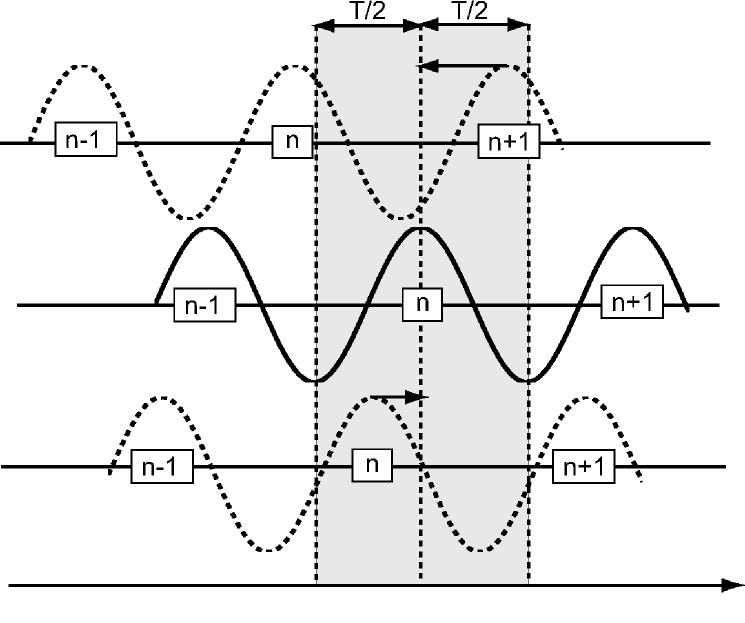
\includegraphics[scale=0.8]{img/ambig_phase.png}
	\caption{Illustration de l'ambiguïté sur la phase (extraite de \cite{brossier_these}). En haut, le déphasage est supérieur à $T/2$, les arches sont mal ajustées. En bas, le déphasage est inférieur à $T/2$, les phases sont bien ajustées. \label{ambig_phase}}
\end{figure}

 Dans cette étude, 

À défaut de disposer à un modèle initial cinématiquement acceptable, il est possible de d'appliquer un ensemble de stratégies permettant de limiter ces artefacts : introduire progressivement les sources ou récepteurs les plus éloignés, rallonger progressivement les temps d'acquisition, et inverser prioritairement les données basses fréquences.


En sismologie, une image issue de tomographie peut fournir un modèle initial assez précis. Dans cette étude, on considère que peu d'informations sont connues sur les paramètres élastiques de la soudure et le modèle initial choisi est uniforme (cf chapitre~\ref{applications}). Cependant, il serait intéressant d'envisager l'utilisation d'un modèle initial construit statistiquement à partir des résultats d'inversion d'un grand nombre de soudure.

\subsection{Inversion multi-paramètres}

Chaque changement de variable donne une nouvelle expression des différentielles des paramètres. 

choix des paramètres à inverser : ils ont différentes amplitudes et différents effets sur le champ d'onde, 
diagramme de rayonnement
citer forgues p.156 \citep{forgues}

\begin{figure}[!h]
	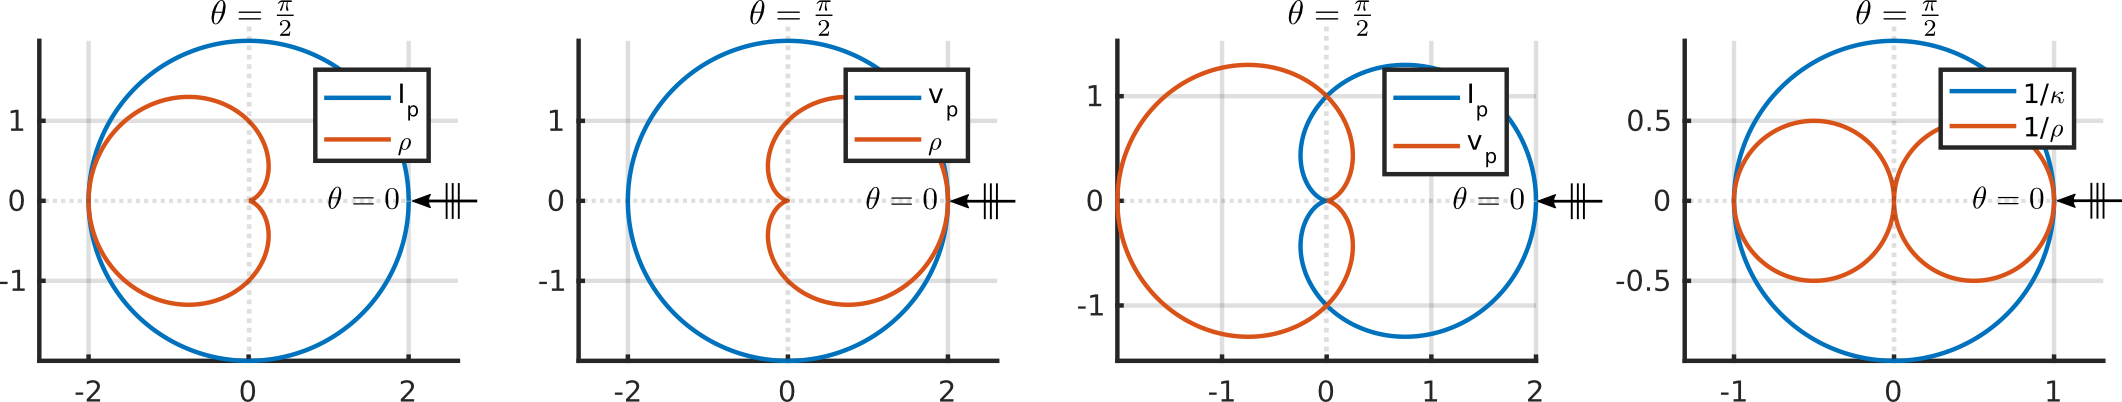
\includegraphics[scale=0.5]{img/rayonnement.png}
	\caption{Diagrammes de rayonnement pour différentes paramétrisations d'un milieu acoustique.\label{rayonnement}}
\end{figure}


\subsection{estimation de la source}






\section{resultats en geophy}

...et aussi appliqué en médical et à des ondes électromagnétiques, rayon X : natterer ?

\section{application au cnd de soudure : les problématiques}

-guide d'onde
-acquisition en surface seulement, et problématique de la soudure bombée
-anisotropie (cf image soudure) forte, qui touche not. les ondes S.
-acquisition horizontale pas idéale pour inverser la vitesse horizontale (car petits offsets et peu de courbure de rayon comme en géophys) (discuter le choix des paramètres à inverser compte-tenu de la configuration)
-sources et récepteurs mobiles 
-geophysique, dispositif de surface, donc on ne considère que les diffractions rayonnant vers la surface (soit angle de diffraction de max 180°)(Forgues, pages 160). En CND, on illumine des deux côté


%\begin{figure}
%	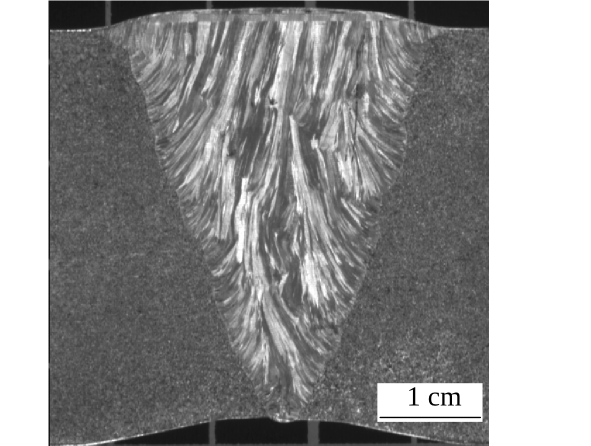
\includegraphics[height=5cm]{./img/soudure1.png}
%	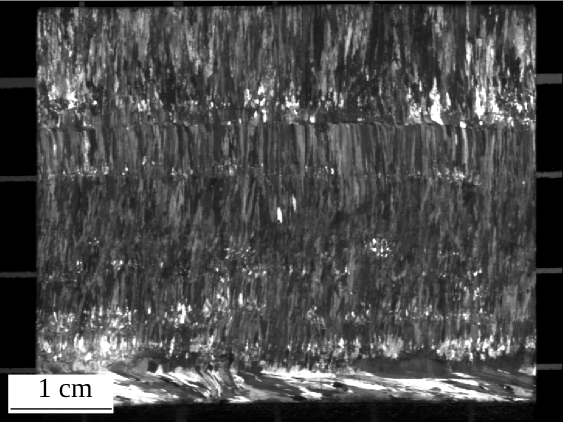
\includegraphics[height=5cm]{./img/soudure2.png}
%	\caption{Macrographie d'une soudure industrielle en acier inoxydable en acier austénitique \citep{chassignole}. À gauche : coupe dans le plan $(x,z)$, à droite : coupe dans le plan $(x,y)$.}
%\end{figure}

grains colonnaires

p91 potel bruneau : données "d'aspect limité" : il n'es tpas possible de tourner autour de l'obstace. On colpense la perte d'info en réalisant les mesures sur plusieurs freq et possibilité de déplacer capteur.




\subsection{sensibilité au bruit ?}

\todo[inline]{Les impasses volontairement faites : \\
	- détail de la discrétisation différences finies / détail des calculs FEM\\	
}


\todo[inline]{born approx}


\chapter{Application de la FWI à des données simulées \label{applications}}

p91 potel bruneau en francais: données "d'aspect limité" : il n'est pas possible de tourner autour de l'obstacle. On compense la perte d'info en réalisant les mesures sur plusieurs freq et possibilité de déplacer capteur.

\section{Génération des données observées}

Les données de référence sont générées par la résolution d'un problème direct.
Le signal d'excitation choisi est une fonction de Ricker qui correspond à la dérivée seconde d'une Gaussienne et qui est définie de la manière suivante : 
\begin{equation}
	s(t)=(1-(t-t_{0}f\pi))^2e^{-((t-t_{0})\pi f)^2}\text{.}
\end{equation}
\todo[inline]{Est-ce réaliste ?}

Deux barrettes de 64 éléments sont utilisées en réception et en transmission. La fréquence centrale d'excitation est 2 MHz.



%\section{Discrétisation}

%Les discrétisations spatiales et temporelles sont contraintes par
%2 conditions sur la discrétisation : 
%CFL et ..points par longueur d'onde pour les schéma d'ordre ... et... (en différences finies)

\section{Analyse de résolution spatiale}
En théorie, si l'éclairage est parfait, on est limité en résolution par lambda/2 (cf review virieux ou thèse de romain : "pouvoir de résolution du gradient"). En pratique, tout comme en ray-tomo (cf wiliamson cité dans review virieux), on est très limité par l'éclairage.

Afin de déterminer le pouvoir de résolution du gradient, \cite{sirgue} réalise une analyse en onde plane comme suit. Considérons une onde plane incidente se propageant vers un point diffractant (suivant $\bm{s}$), donnant naissance en ce point à une autre onde plane se propageant suivant $\bm{r}$ (cf figure~\ref{}).\todo[inline]{pourquoi pas vers le récep ? i e Sirgue 2004 p.3 : pourquoi tous ces conjugués ?}

\begin{equation}
	k= \frac{\omega}{c} 2 \cos\left( \frac{\theta}{2}\right)
\end{equation}

La résolution est donc maximale quand $\theta=0$ et elle est alors de $\lambda/2$. La résolution s'améliore en hautes fréquences et pour des petits angles de diffraction. La géométrie du système d'acquisition a donc un impact direct sur la résolution spatiale. De plus, les surfaces libres simulent la présence de sources miroirs, d'autant plus nombreuses que le nombre de réflexions dans le guide est important. \\


supposés sans interaction

Une illustration du lien entre la couverture en nombres d'onde du milieu et l'acquisition ainsi que les sources miroirs est réalisée ci-après. Pour différentes configurations, des transformée de Fourier spatiales du gradient sont réalisées au niveau de dix-huit points diffractant, le paramètre du modèle étant la vitesse verticale (cf figure~\ref{app:config_reso}).

\begin{figure}
	\centering
	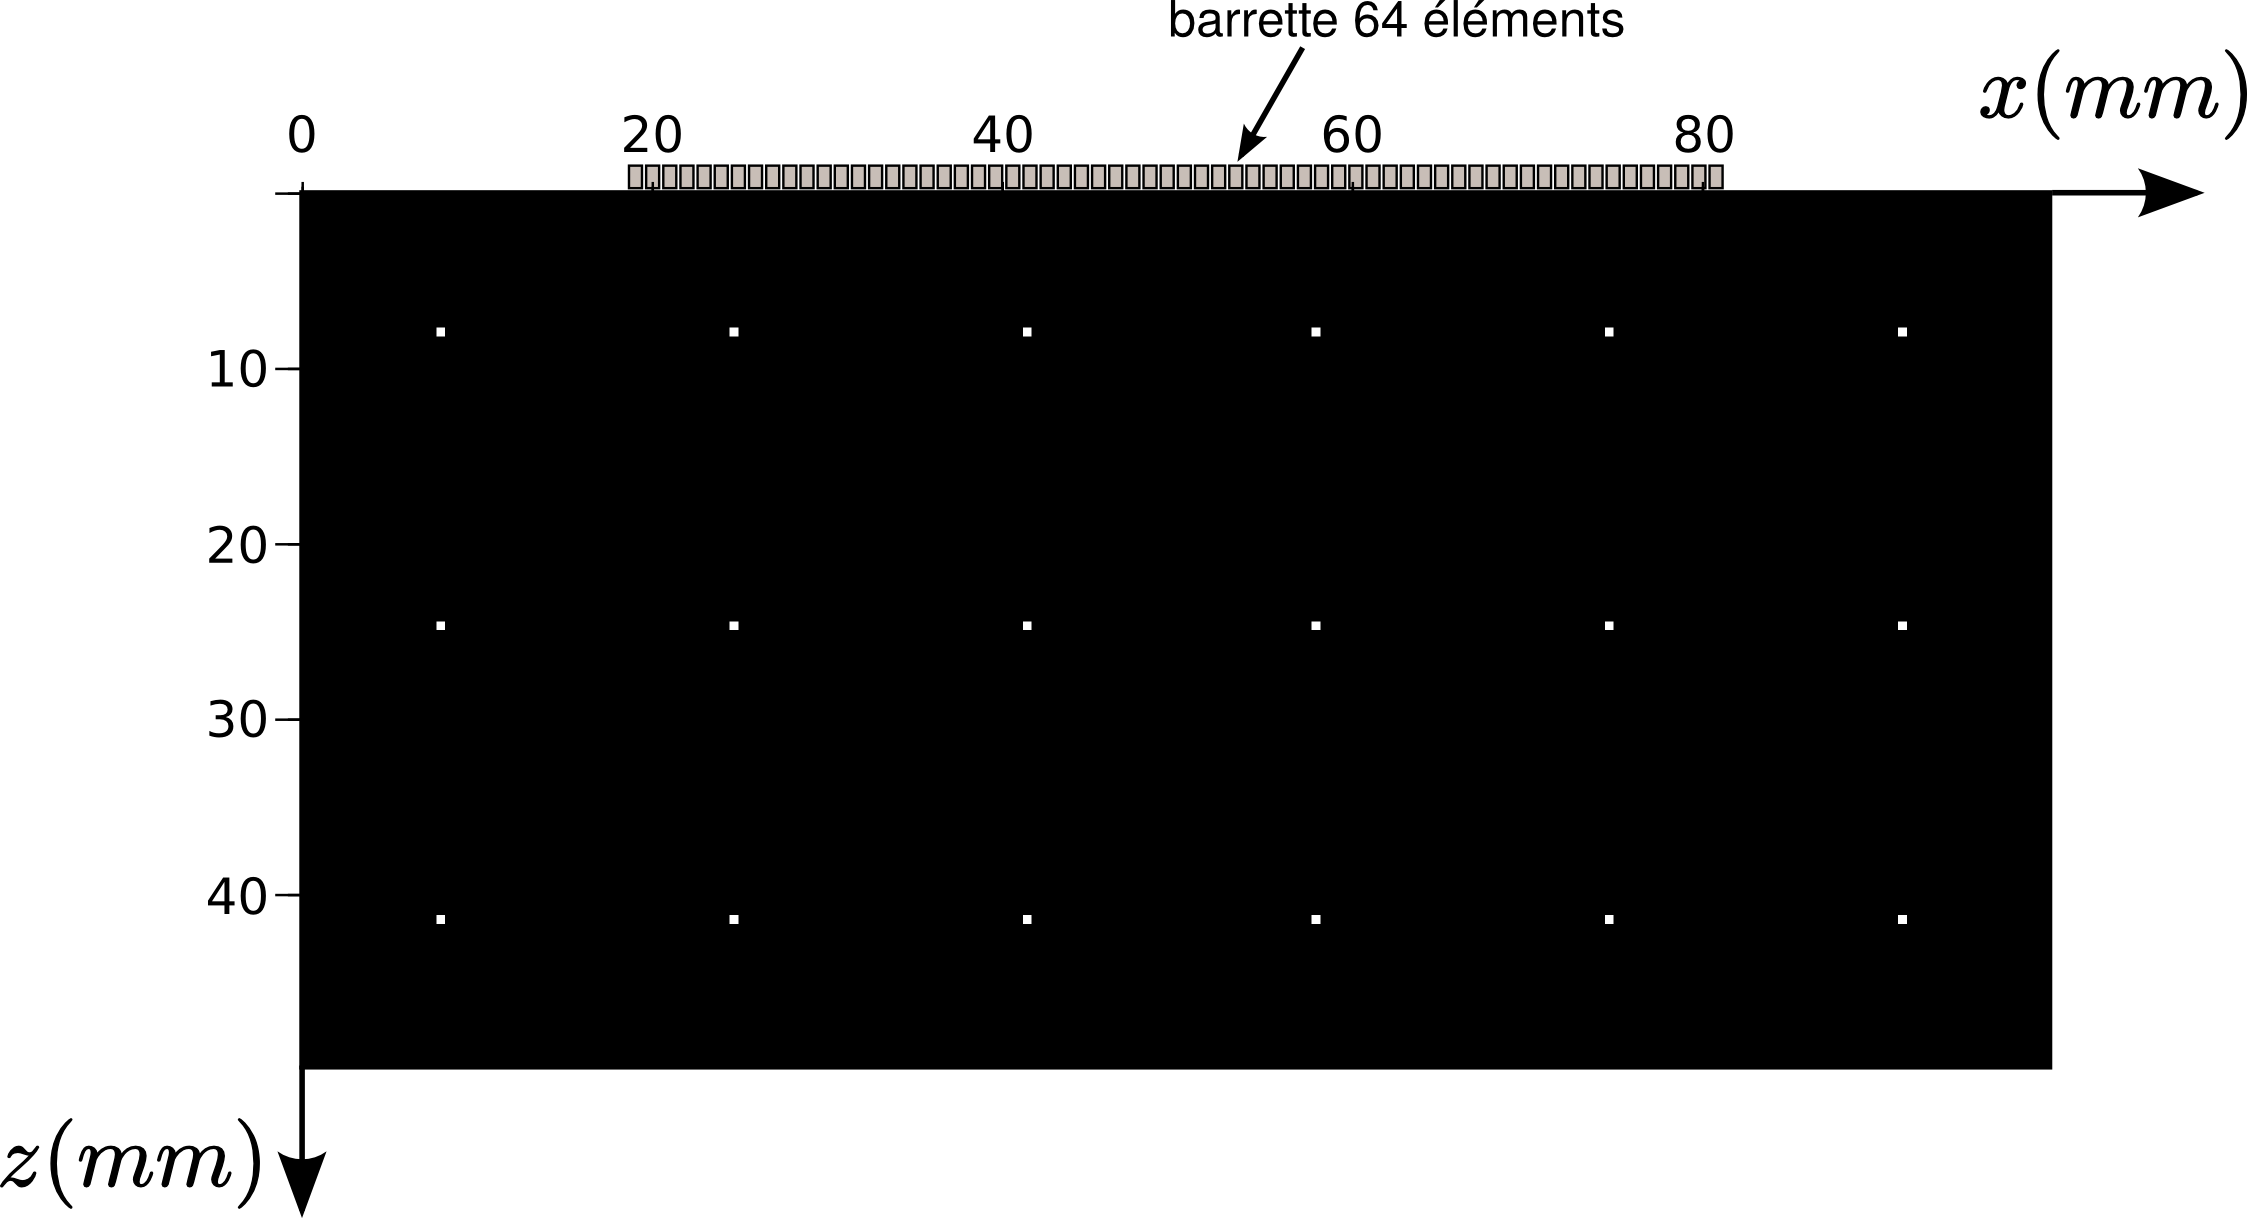
\includegraphics[height=5cm]{img/vp_scat.png}
	\caption{Configuration pour l'étude de résolution. La vitesse dans les inclusions est de 3000 m/s et de 6000 m/s ailleurs. \label{app:config_reso}}
\end{figure}

Le gradient est calculé en présence des dix-huit inclusions, sous l'hypothèse pour chaque inclusion, que la présence des autres n'intervient pas.\todo[inline]{à reformuler}

\subsection{Influence de la fréquence d'excitation}

Dans un premier temps, le milieu est entouré de conditions absorbantes. Les figures~\ref{app:150k} et~\ref{app:2M} montre la couverture en nombre d'onde obtenue dans une configuration avec une barrette excitatrice et pour deux gammes de fréquence différentes. 
    
\begin{figure}[!h]
    \centering
    \begin{subfigure}[b]{0.05\textwidth}
 		\hspace{-2cm}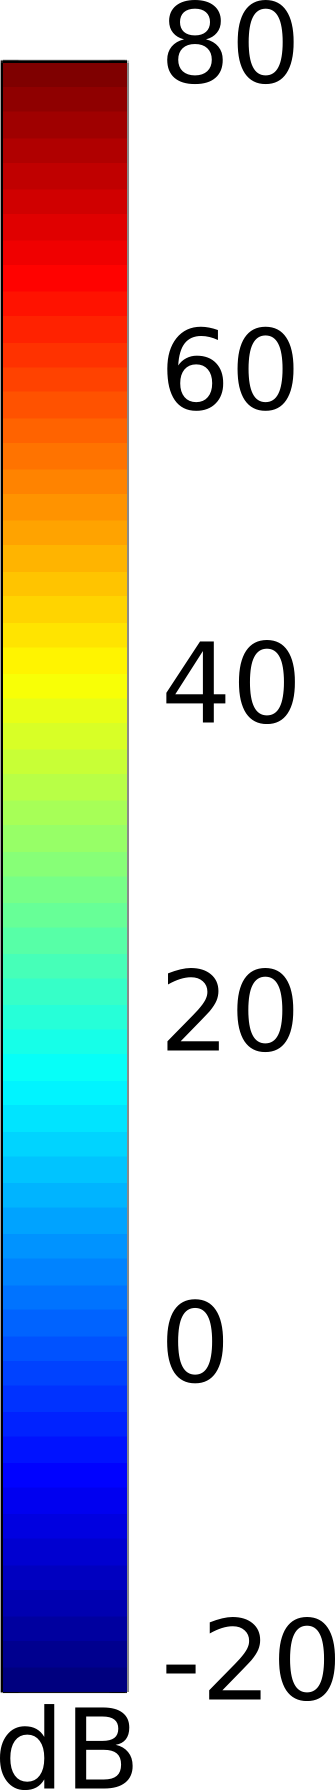
\includegraphics[width=0.5cm]{img/echelle_fft.png}\vspace{2.1cm}
	\end{subfigure}
    \begin{subfigure}[b]{0.4\textwidth}
		\hspace{-3cm}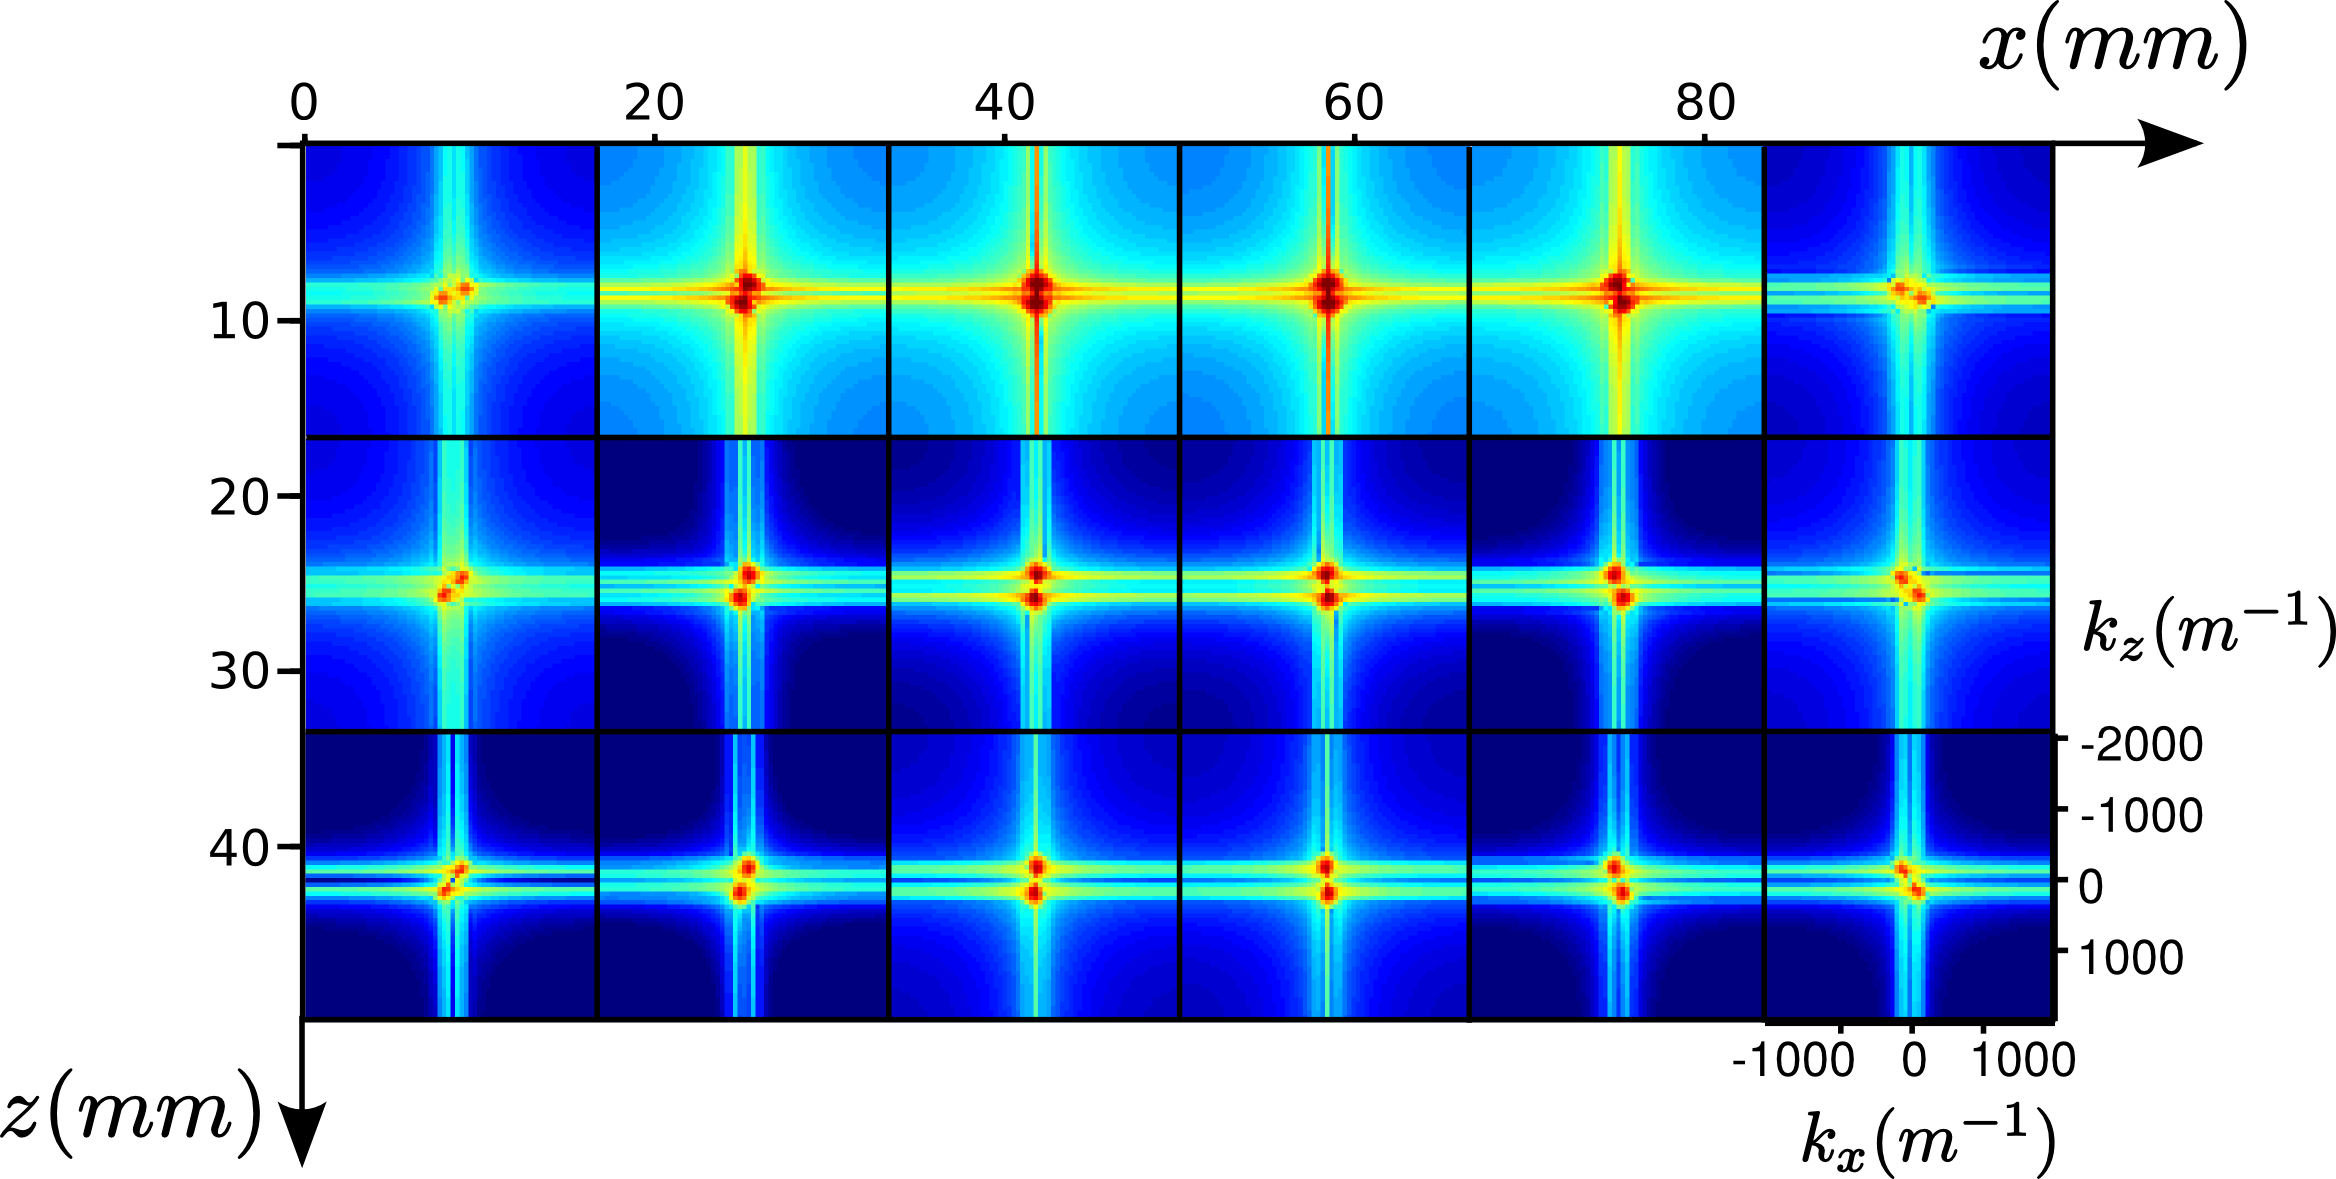
\includegraphics[width=1.5\textwidth]{img/ssfreesurf_150k}
		\caption{Excitation centrée à 150 kHz.}
		\label{app:150k}
	\end{subfigure}	
	%\hspace{0.7cm}
	\begin{subfigure}[b]{0.4\textwidth}
		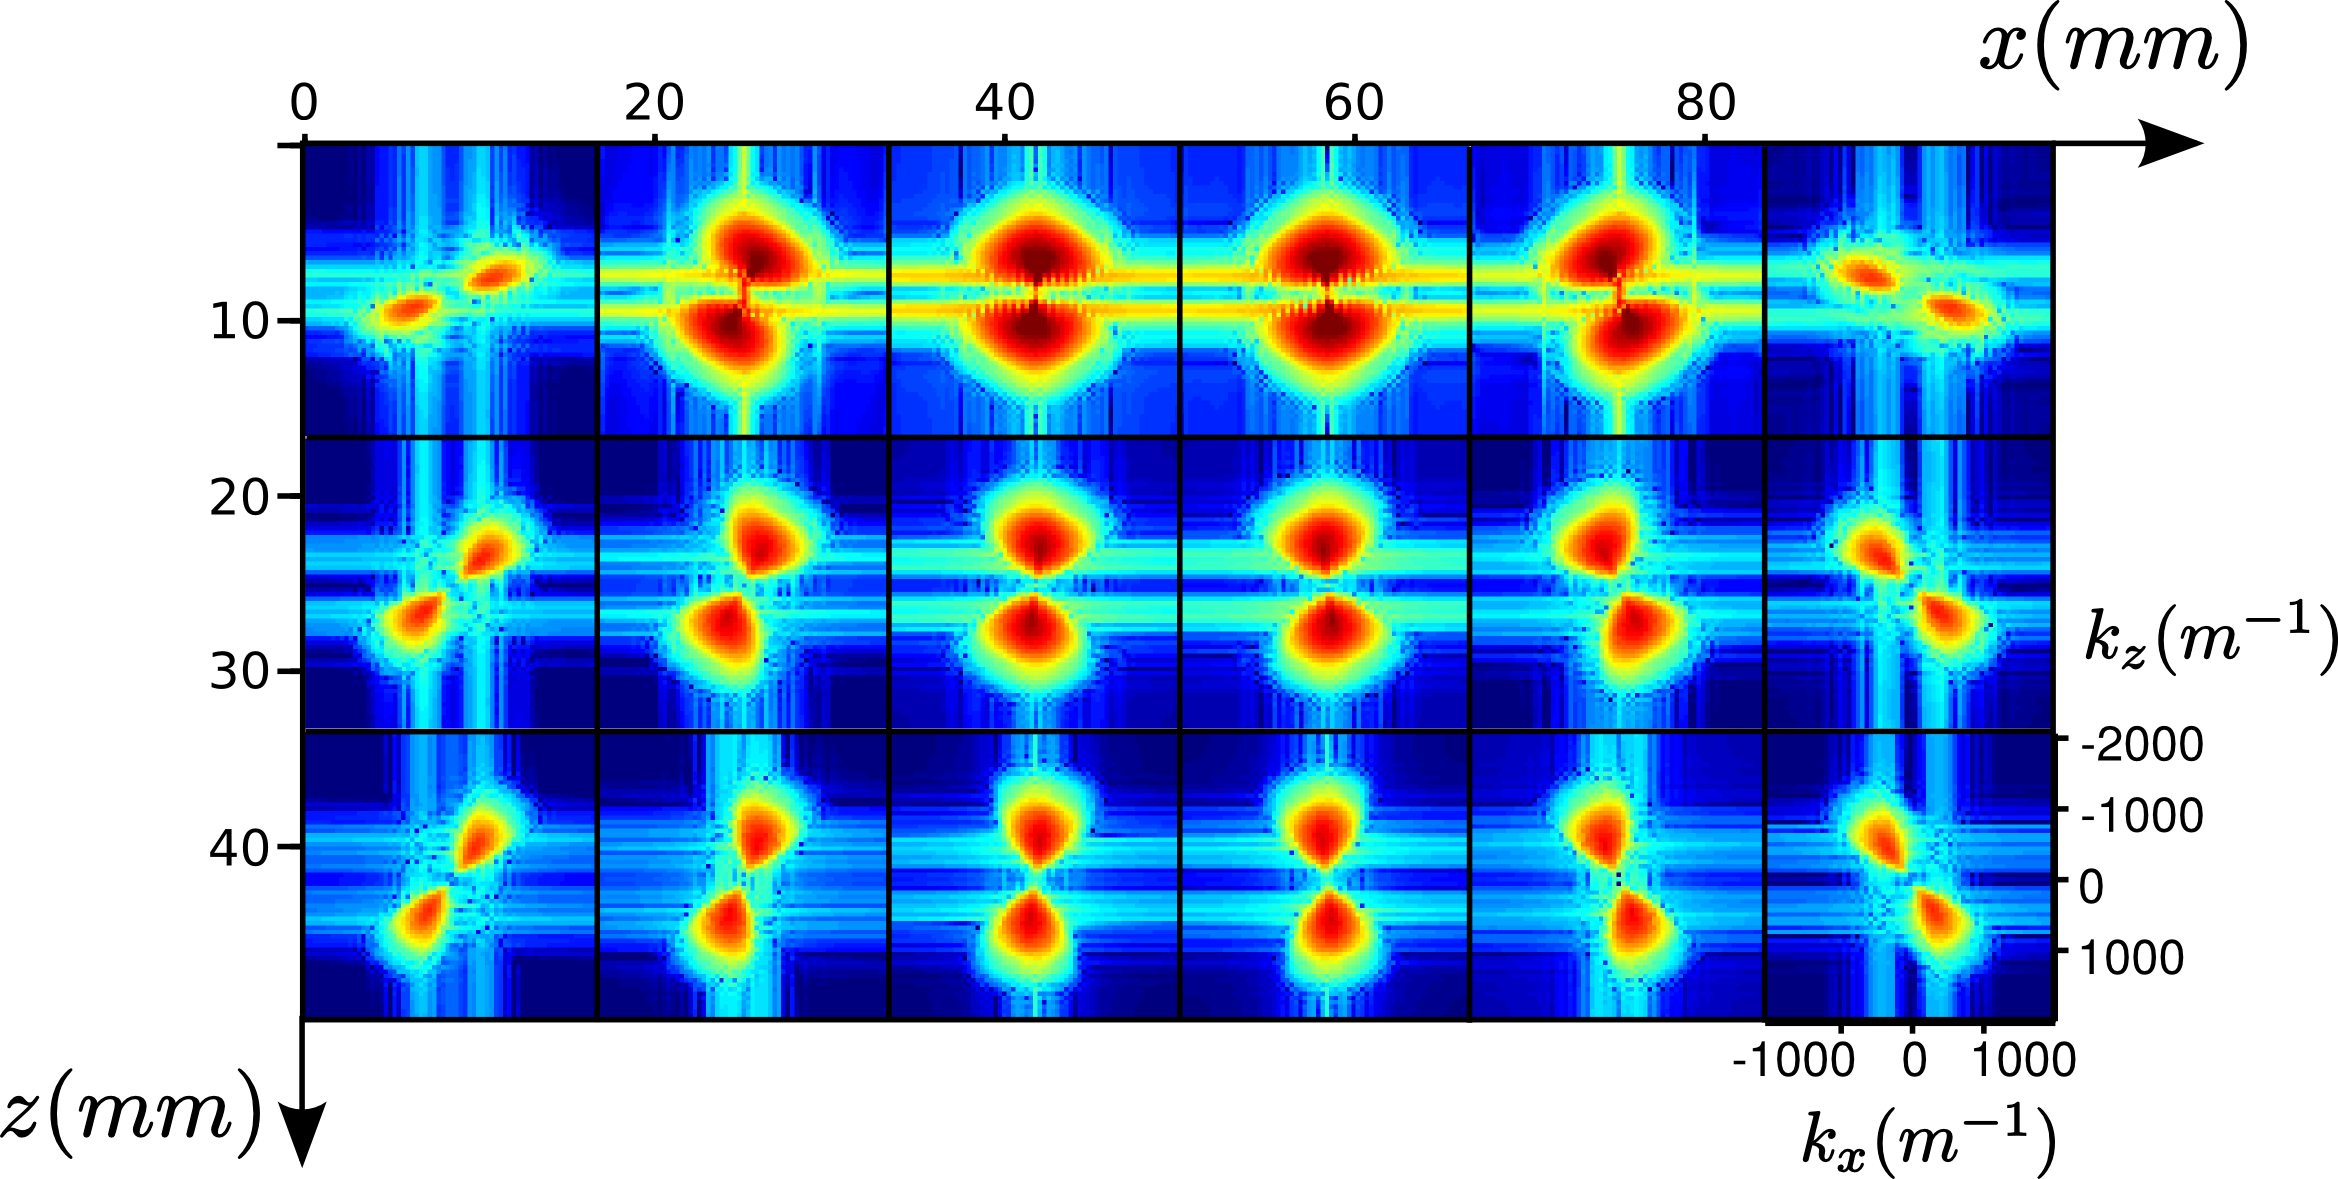
\includegraphics[width=1.5\textwidth]{img/ssfreesurf_2M}
		\caption{Excitation centrée à 2 MHz.}
		\label{app:2M}
	\end{subfigure}
	\caption{Transformées de Fourier spatiales locales pour 2 gammes de fréquence d'excitation.}
\end{figure}

Dans le cas d'une excitation basse fréquence, le gradient est pauvre en hauts nombres d'onde. Inversement, l'excitation haute fréquence ne permet pas de reconstruire les bas nombres d'onde.\\
La couverture en nombre d'onde est également très liée à l'acquisition. Elle est meilleure aux abords et en direction de la barrette. Les nombres d'onde verticaux seront globalement mieux reconstruits avec cette acquisition, tandis que la couverture en nombres d'ondes horizontaux est très faible.

\subsection{Influence des surfaces libres}


\section{Gestion des non-linéarités}
Une stratégie pour limiter la non-linéarité de l'inversion consiste à réaliser l'inversion en plusieurs temps, en injectant progressivement le contenu haute fréquence dans les données. L'inversion à basse fréquence permet ainsi de reconstruire la structure grossière avant d'ajouter les détails grâce à la résolution qu'offre le gradient en haute fréquence.\\



Afin que les nombres imagés soient correctement échantillonnés, il faut que le plus grand nombre d'onde imagé à une fréquence soit le même que que le plus petit à la fréquence suivante \citep{sirgue}. En considérant que le plus nombre d'onde est obtenu pour une angle de diffraction de $\pi/2$ , le rapport de fréquences suivant doit donc être respecté : 

\begin{alignat*}{3}
	  ~&k_{max}(f_{n}) &&= k_{min}(f_{n+1})\\
	\Leftrightarrow~~~~~ &  f_n &&= f_{n+1}\cos \left(\frac{\pi}{2} \right)\\
	 \Leftrightarrow~~~~~ & \frac{f_{n+1}}{f_n} && \approx  1,5.
\end{alignat*} 

Les inversions présentées ci-après sont donc réalisées en plusieurs itérations. Entre chaque itérations, les données observées et l'ondelette d'excitation sont filtrées par un filtre passe-bas de fréquence centrale $f_{n}$ et dont la fréquence de coupure haute est de $2,5 \times f_{n}$.


\section{Équations de propagation pour le problème direct}

La propagation des ondes élastiques est décrite par les équations linéarisées en déplacements $\bm{u}$ et contraintes $\bar{\bar T}$ suivantes \citep{mat_ac} : 

\begin{eqnarray}
	\rho \frac{\dd^2 u_{i}}{\dd t^2} &=& \displaystyle\sum_{j}\frac{\dd T_{ij}}{\dd x_{j}}\\
	T_{ij}&=&C_{ijkl}\left( \frac{\dd u_{i}}{\dd x_{j}} + \frac{\dd u_{j}}{\dd x_{i}}\right)\text{,}
	\label{prop}
\end{eqnarray}
avec $C_{ijkl}$ le tenseur des constantes élastiques.

\subsection{Propagation acoustique}
Les équations de la propagation acoustique peuvent être déduite de~\ref{prop} en considérant un module de cisaillement nul. on a alors $T_{ij}=0$ si $i\neq j$.

\subsubsection{Isotrope}
Dans un milieu isotrope, les constantes élastiques sont égales dans toutes les directions. En milieu acoustique isotrope, les propriétés élastiques sont donc réduites à une seule constante et les équations~\ref{prop} deviennent : 
\begin{eqnarray}
	\rho \frac{\dd^2 u_{i}}{\dd t^2} = -\bm{\nabla} p\\
	p=-\kappa \displaystyle\sum_{i} \frac{\dd u_{i}}{\dd x_{i}}\text{,}
\end{eqnarray}
avec $\kappa$ le module de rigidité et $p$ la pression.

\subsubsection{Transverse isotrope}

Il est possible de formuler à partir de~\ref{prop} des équations d'ondes acoustiques en milieu anisotrope. Bien que ce soit physiquement impossible, cette formulation permet de se rapprocher cinématiquement des équations d'ondes élastiques, de manière simplifiée \citep{alkhalifah}.

Notons que cette formulation [Pose quelques problèmes (Duveneck 2008) notamment génération d'onde S (sur données "vrai simulée"  et sur problème direct, mais pas la même car différente grille, PML, ... donc on la mute sur le résidu) qui n'a pas de sens physique. Proposer les solutions (taper Epsilon, en sismo on est dans l'eau donc c'est fait naturellement -> placer les sources dans un milieu isotrope).]
 

La paramétrisation du milieu est faite à l'aide des constantes de Thomsen~\citep{thomsen} surtout utilisées dans le domaine des Sciences de la Terre définies comme suit : 
\begin{eqnarray}
	\epsilon & =  & \frac{C_{11}-C_{33}}{2C_{33}} = \frac{\bm{v}_{p}.\bm{e}_{x} -  \bm{v}_{p}.\bm{e}_{z}}{\bm{v}_{p}.\bm{e}_{z}}\\
	\delta & = & \frac{(C_{13}+C_{44})^2-(C_{33}-C_{44})^2}{2C_{33}(C_{33-C_{44}})}\text{.}\\
\end{eqnarray}
+theta

Le paramètre $\epsilon$ est donc lié à la différence entre la composante verticale et la composante horizontale de la vitesse des onde de pression et $\delta$ décrit davantage la propagation des ondes quasi-longitudinales.



\section{Inversions en matériau acoustique }

Dans un premier temps, la méthode d'imagerie est appliquée à des milieux acoustiques, ce qui simplifie le problème et réduit les coût de calcul. Les études proposées dans cette section sont menées en approximation 2D : on suppose que le problème ne dépend pas du tout de la dimension données par $\bm{e}_{y}$.\\

Le code utilisé est \emph{TOYxDacTIME} développé dans le cadre du projet \emph{Seiscope}\footnote{http://seiscope2.osug.fr}. Le problème direct y est résolu par différences finies, ce qui contraint 

\subsection{Isotrope}




monoparamètre : vp
multi paramètre ?



\subsection{VTI}
Afin d'introduire une anisotropie simplifiée dans la soudure, une étude dans un milieu acoustique VTI est menée.\\

On considère une plaque isotrope dans laquelle se trouve une soudure anisotrope VTI sans défaut. On cherche à évaluer l'influence de l'anisotropie en vue d'inverser le paramètre $\epsilon$. La valeur de $\epsilon$ dans la soudure est fixée à 20\%, ce qui est environ deux fois plus élevé que les valeurs que l'on peut trouver dans la littérature~\citep{chassignole}. Les deux barrettes excitatrices/réceptrices sont placées de manière éloignée, afin d'accentuer la propagation des ondes suivant $\bm{e}_{x}$ et de s'assurer que les temps de vol soient perturbés par l'anisotropie (figure~\ref{configuration_vti}).\\
Les autres paramètres ($v_{p}$,$\rho$ et $\delta$) sont supposés constants et uniformes.\\

Une comparaison des données observées en milieu isotrope ($\epsilon = 0$) et avec la soudure anisotrope est proposée en figure~\ref{}. Il apparaît que la présence d'une anisotropie VTI a peu d'impact sur les données, car le dispositif d'acquisition favorise la mesure des ondes dont le trajet est majoritairement vertical et donc peu perturbé.\\
 L'inversion du paramètre $\epsilon$ est alors difficile : une modification grossière de la vitesse horizontale suffit à corriger les retards résiduels (cf figure~\ref{}).
 
 \todo[inline]{figures : configurations ; traces isotrope, epsilon=20 ; inversion + données calculées}
 
Un modèle de soudure anisotrope VTI est donc trop simple pour représenter l'anisotropie d'une soudure réelle, dont on sait qu'elle impacte beaucoup le faisceau ultrasonore. Pour tester la capacité de la FWI à reconstruire ces paramètres d'anisotropie, il est donc nécessaire d'utiliser un modèle plus pertinent qui se rapprocherait davantage de celui proposé par \cite{ogilvy} par exemple.\\

Le modèle proposé par \cite{ogilvy} est de la forme : 
\begin{equation}
	\theta(x,z) = \tan^{-1}\left( \frac{D/2 + z\tan\alpha}{x} \right),
\end{equation}
avec $D$ la largeur de la racine de la soudure et $\alpha$  l'angle du bord de soudure.

 Conclusion : inversion de $\epsilon$ -> dur et par pertinent
passer en tilted (façon ogilvy ?) ou modèle plus précis en élastique.

\section{Inversions en matériau élastique isotrope}




%%%%%%%%%%%%%%%%%%%%%notes%%%%%%%%%%%%%%%
\todo[inline]{notes : }
\subsection{anisotrope}

anisotrope est plus problématique que isotrope car : 
-modélisation plus complexe,
-problème moins bien posé

Gholami 2011 : la vitesse a beaucoup plus d'influence sur les données que les paramètres delta et epsilon (delta étant le plus faible). D'après ses schémas, on va donc avoir une maj de la vitesse mais pas des autres paramètres

modèle initial de soudure : citer mina ?

%VTI elliptique ne gène pas l'inversion car beaucoup d'info portées par la transmission (vecteurs d'ondes verticaux non affectés par l'anisotropie elliptique VTI)  -> pas assez proche du modèle réel

%le flop du vti montre que l'inversion des paramètres est tributaire de l'acquisition

Romain : passer en TTI (code en freq)





%%%%%%%% Biblio %%%%%%%%%%
\newpage

\bibliographystyle{plainnat}%\bibliographystyle{unsrt}
\bibliography{biblio}

\end{document} % fin doc


